\section{Experiments}
\label{sec:experiments}

\subsection{Experimental Setting}
\label{subsec:setting}

We evaluate six agents on 1,017 test scenarios from \benchmark{} using three base language models: Gemini-3-Flash, GPT-5-mini, and Solar-Pro3. All models use temperature 0.7 with a maximum of 10 interaction turns per scenario.

Evaluation employs a multi-judge protocol using two LLMs from different providers: GPT-4o-mini (OpenAI) and Gemini-2.5-flash-lite (Google). This cross-provider design mitigates potential self-preference bias where models may favor outputs from the same provider. Final scores are computed using median aggregation across judges to ensure robustness.

%% Figure: Theoretical quality analysis (placed here for earlier page placement)
\begin{figure*}[!t]
\centering
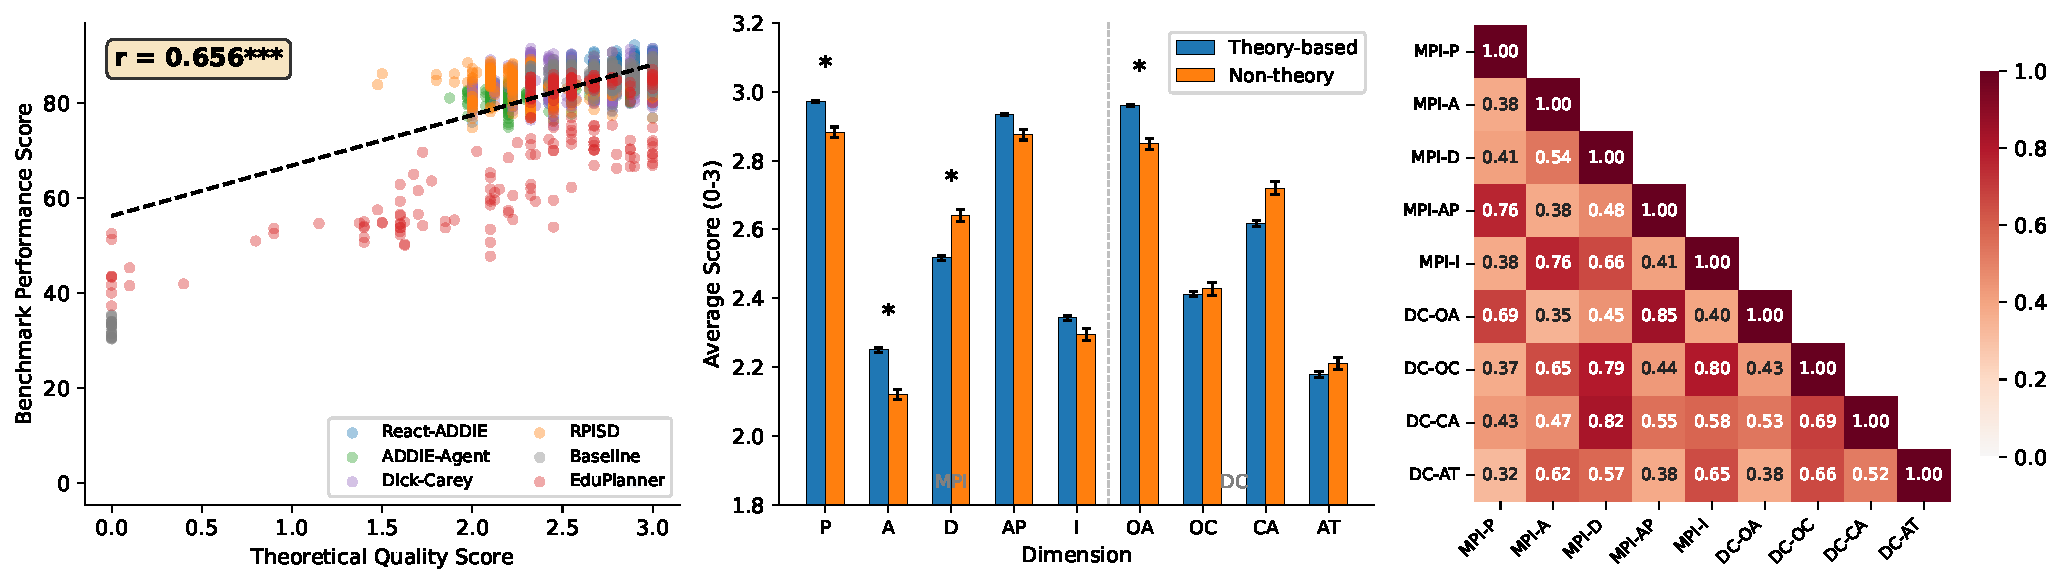
\includegraphics[width=\textwidth]{fig_paper_findings_1_3.pdf}
\caption{Theoretical quality analysis. \textit{Left panel} shows correlation between theoretical quality scores and benchmark performance ($r = 0.656$, $p < 0.001$). \textit{Middle panel} compares theory-based and non-theory agents across all 9 dimensions, where asterisks indicate significant differences ($d > 0.2$). \textit{Right panel} displays inter-dimension correlation matrix revealing cross-framework relationships.}
\label{fig:findings-1-3}
\end{figure*}

